\documentclass[11pt,a4paper]{article}
\usepackage[utf8]{inputenc}
\usepackage[T1]{fontenc}
\usepackage{charter}
\usepackage[scaled=0.92]{helvet}
\usepackage{courier}
\usepackage{amsmath,amssymb}
\usepackage[a4paper,top=2.6cm,bottom=2.6cm,left=2.5cm,right=2.5cm,headheight=14pt]{geometry}
\usepackage{xcolor}
\usepackage{graphicx,booktabs,tabularx,array,float,enumitem,microtype}
\usepackage{titlesec,fancyhdr,lastpage}
\usepackage[most]{tcolorbox}
\usepackage[font=small,labelfont={bf,sf,color=verde},labelsep=period]{caption}
\usepackage[colorlinks=true,linkcolor=verde,urlcolor=verde]{hyperref}

\definecolor{verde}{HTML}{1F4E99}
\definecolor{gris}{HTML}{5F6B6D}
\definecolor{lineagris}{HTML}{B9C3C5}

% Sin patrones de silabeo en español en este entorno: se evita partir palabras
\hyphenpenalty=10000 \exhyphenpenalty=10000 \emergencystretch=3em \tolerance=2000
\renewcommand{\figurename}{Figura}
\renewcommand{\tablename}{Tabla}
\renewcommand{\contentsname}{Índice}

% Títulos de sección: sans serif en color, con una línea gris debajo; cada sección empieza en página nueva
\titleformat{\section}{\sffamily\LARGE\bfseries\color{verde}}{\thesection}{0.8em}{}[\vspace{2pt}{\color{lineagris}\titlerule[0.8pt]}]
\titleformat{\subsection}{\sffamily\large\bfseries\color{verde}}{\thesubsection}{0.7em}{}
\titlespacing*{\section}{0pt}{28pt}{14pt}
\titlespacing*{\subsection}{0pt}{14pt}{4pt}
\usepackage{needspace}
\newcommand{\sectionbreak}{\Needspace{10\baselineskip}}

\pagestyle{fancy}
\fancyhf{}
\fancyhead[L]{\sffamily\footnotesize\color{gris}Agentes inteligentes en un escenario basado en \emph{Apocalypse Now}}
\fancyhead[R]{\sffamily\footnotesize\color{gris}Fundamentos de Inteligencia Artificial}
\fancyfoot[R]{\sffamily\footnotesize\color{gris}Página \thepage\ de \pageref{LastPage}}
\renewcommand{\headrule}{{\color{lineagris}\hrule height 0.4pt}}

\setlength{\parindent}{0pt}
\setlength{\parskip}{6pt}
\setlist{itemsep=2pt,topsep=3pt}
\newcommand{\code}[1]{\texttt{#1}}

\begin{document}

% ================= Portada (con resumen) =================
\begin{titlepage}
\sffamily
{\color{gris}\small UNIVERSIDAD PONTIFICIA COMILLAS · ICAI\\[2pt]
Grado en Ingeniería Matemática e Inteligencia Artificial}

\vspace{2.6cm}
\begin{tcolorbox}[enhanced,frame hidden,colback=white,borderline west={5pt}{0pt}{verde},left=16pt,top=6pt,bottom=6pt]
{\color{gris}\large Fundamentos de Inteligencia Artificial · Proyecto final}\\[12pt]
{\fontsize{26}{32}\selectfont\bfseries\color{verde} Agentes inteligentes en un escenario\\[4pt] basado en \emph{Apocalypse Now}}\\[14pt]
{\Large Agente lógico, agente bayesiano y proceso de decisión de Markov}
\end{tcolorbox}

\vspace{1.4cm}
{\rmfamily\small
{\sffamily\bfseries\color{verde} Resumen}\par\smallskip
Este proyecto modela la misión del Capitán Willard, inspirada en la película \emph{Apocalypse Now}, mediante tres agentes de inteligencia artificial. En la primera parte, un \textbf{agente lógico} con base de conocimiento guía al jugador por un palacio de $6\times6$ casillas con precipicios, un soldado y una salida ocultos. En la segunda, un \textbf{agente bayesiano} mantiene distribuciones de probabilidad sobre la posición de tres trampas, el soldado y la salida, las actualiza con la regla de Bayes y recomienda los movimientos cuyo riesgo es inferior a un umbral. En la tercera, el cruce de un río con corriente se formula como un \textbf{proceso de decisión de Markov} y se resuelve con \emph{value iteration}. Los dos primeros agentes asisten a un jugador humano, que es quien decide cada acción; el tercero calcula una política óptima y la simula de forma autónoma.\par}

\vfill
{\color{lineagris}\rule{\linewidth}{0.8pt}}\\[8pt]
\begin{tabularx}{\linewidth}{@{}lX@{}}
\textbf{Autor} & Jaime Tuesta de Simón\\[3pt]
\textbf{Curso} & 2.º del Grado en Ingeniería Matemática e Inteligencia Artificial\\[3pt]
\textbf{Fecha} & Enero de 2026\\
\end{tabularx}
\end{titlepage}

% ================= Índice (página propia) =================
\begingroup
\renewcommand{\sectionbreak}{}
\titleformat{\section}{\sffamily\LARGE\bfseries\color{verde}}{}{0pt}{}[\vspace{2pt}{\color{lineagris}\titlerule[0.8pt]}]
\tableofcontents
\endgroup
\clearpage

% ================= 1 =================
\section{Introducción}

El proyecto representa la misión del Capitán Willard para localizar al Coronel Kurtz y escapar con él. Se divide en tres programas independientes, que se resumen en la Tabla~\ref{tab:programas}.

\begin{table}[H]
\centering\small
\caption{Programas del proyecto.}\label{tab:programas}
\begin{tabularx}{\linewidth}{@{}l>{\raggedright\arraybackslash}p{3.6cm}X@{}}
\toprule
\textbf{Programa} & \textbf{Técnica} & \textbf{Problema}\\
\midrule
\code{kurtz.py} & Agente lógico con base de conocimiento & Palacio con tres precipicios, un soldado dormido, Kurtz y la salida.\\
\code{palacio.py} & Agente bayesiano & Palacio con tres trampas (fuego, pinchos y dardos), un soldado, Kurtz y la salida.\\
\code{river\_mdp.py} & MDP y \emph{value iteration} & Cruce de un río con corriente e islas hasta la salida.\\
\bottomrule
\end{tabularx}
\end{table}

En los dos escenarios del palacio se sigue la primera de las opciones del enunciado: un jugador controla a Willard, y el agente le presenta en cada turno la información que ha inferido, le indica qué casillas son seguras y hacia dónde debe dirigirse. En el escenario del río, el agente calcula una política óptima y la ejecuta por sí mismo.

% ================= 2 =================
\section{Entorno del palacio}

\subsection{Estructura}
El palacio se modela como una cuadrícula de $6\times6$ casillas generada aleatoriamente en cada ejecución. Willard empieza siempre en la casilla $(0,0)$ y el resto de elementos se colocan al azar (Tabla~\ref{tab:elementos}). Todas las casillas están ocultas al principio: el jugador solo ve las casillas que ha visitado.

\begin{table}[H]
\centering\small
\caption{Elementos del palacio en cada parte.}\label{tab:elementos}
\begin{tabularx}{\linewidth}{@{}lXX@{}}
\toprule
 & \textbf{Parte 1: agente lógico} & \textbf{Parte 2: agente bayesiano}\\
\midrule
Peligros & 3 precipicios (P), letales & 3 trampas: fuego (F), pinchos (P) y dardos (D), letales; pueden coincidir en una casilla\\
Soldado & S: mata a Willard; puede morir con la granada & M: igual que en la parte 1\\
Kurtz & K: hay que rescatarlo antes de salir & K: igual que en la parte 1\\
Salida & E & S\\
Restricciones & Cada elemento ocupa una casilla vacía & Ningún elemento en $(0,0)$; el soldado, Kurtz y la salida nunca están en una casilla con trampa\\
\bottomrule
\end{tabularx}
\end{table}

\subsection{Acciones}
El jugador dispone de tres tipos de acción:
\begin{itemize}
\item \textbf{Moverse} (\code{W}, \code{A}, \code{S}, \code{D}), con \code{move\_captain()}. Willard muere si entra en una casilla con un peligro o con el soldado vivo, y rescata a Kurtz automáticamente al entrar en su casilla.
\item \textbf{Lanzar la granada} (\code{G}) a una casilla adyacente, con \code{throw\_grenade()}. Si acierta, el soldado muere; solo hay una granada.
\item \textbf{Salir} (\code{E}), con \code{exit\_palace()}. El juego termina con éxito si Willard está en la salida y ha rescatado a Kurtz.
\end{itemize}

\subsection{Perceptos}
En cada turno, \code{get\_percepts()} devuelve un diccionario de booleanos calculado a partir de las casillas adyacentes a Willard (arriba, abajo, izquierda y derecha), resumido en la Tabla~\ref{tab:perceptos}.

\begin{table}[H]
\centering\small
\caption{Perceptos de cada parte.}\label{tab:perceptos}
\begin{tabularx}{\linewidth}{@{}lX@{}}
\toprule
\textbf{Parte 1 (8 perceptos)} & \textbf{Parte 2 (10 perceptos)}\\
\midrule
Brisa: algún precipicio adyacente & \code{eF}, olor a queroseno: fuego adyacente\\
Ronquido: soldado adyacente & \code{eP}, crujido: pinchos adyacentes\\
Resplandor: salida adyacente o en la casilla actual & \code{eD}, cables en el suelo: dardos adyacentes\\
 & \code{eM}, ronquido: soldado adyacente\\
 & \code{eS}, resplandor: salida adyacente\\
\midrule
\multicolumn{2}{@{}p{\dimexpr\linewidth-\tabcolsep\relax}@{}}{En ambas: \code{Pared\_U}, \code{Pared\_D}, \code{Pared\_L}, \code{Pared\_R} (paredes) y \code{Grito} (la granada ha matado al soldado).}\\
\bottomrule
\end{tabularx}
\end{table}

\begin{figure}[H]
\centering
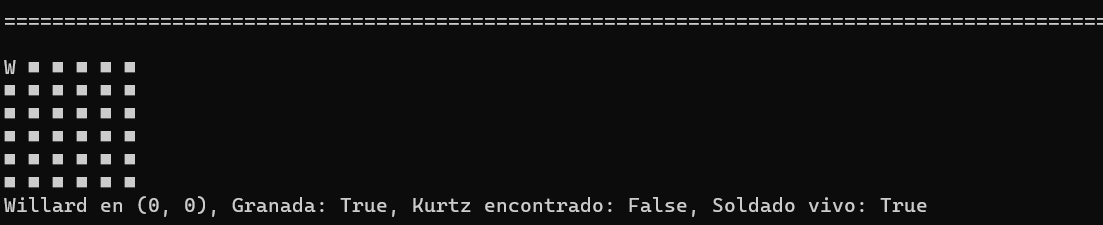
\includegraphics[width=0.62\linewidth]{figs/p1_cuadricula_inicial.png}\hfill
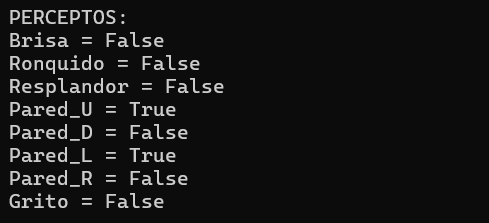
\includegraphics[width=0.3\linewidth]{figs/p1_perceptos.png}
\caption{Parte 1: cuadrícula al inicio de la partida (izquierda) y perceptos del primer turno (derecha).}
\end{figure}

% ================= 3 =================
\section{Parte 1: agente lógico}

\subsection{Base de conocimiento}
La base de conocimiento (KB) se almacena en la clase \code{GameState} y está formada por las siguientes listas:
\begin{itemize}
\item \code{visited}: casillas visitadas.
\item \code{history}: casillas visitadas junto con los perceptos recibidos en cada una.
\item \code{possible\_P}, \code{possible\_S}, \code{possible\_E}: posibles ubicaciones de los precipicios, del soldado y de la salida. Empiezan con todas las casillas y se reducen a medida que se obtiene información.
\item \code{confirmed\_P}: precipicios cuya ubicación se conoce con certeza. Es necesaria porque, al haber tres precipicios, saber que una casilla lo es no permite descartar las demás.
\end{itemize}

\subsection{Inferencia}
La función \code{update\_kb()} recorre el historial en cada turno y aplica las siguientes reglas de inferencia proposicional:
\begin{itemize}
\item Toda casilla visitada es segura: no contiene precipicios ni soldado. Mientras no se haya encontrado la salida, tampoco puede ser la salida.
\item La ausencia de brisa, ronquido o resplandor descarta el elemento correspondiente en todas las casillas adyacentes.
\item Un ronquido o un resplandor restringen las posibles ubicaciones del soldado o de la salida a las casillas adyacentes. Al ser elementos únicos, la información de varios turnos se combina por intersección.
\item La brisa no permite descartar casillas, porque puede deberse a cualquiera de los tres precipicios. Si en la casilla actual hay brisa y solo queda una casilla adyacente que pueda ser precipicio, esa casilla se confirma como precipicio.
\item Una granada fallida descarta la casilla objetivo como posición del soldado.
\end{itemize}

\subsection{Flujo de ejecución e interfaz}
La función \code{main()} ejecuta un bucle en el que cada iteración es un turno: se imprime el tablero y el estado de Willard, se calculan y muestran los perceptos, se actualiza la KB y se muestran las inferencias, y se pide al jugador la siguiente acción. El bucle termina cuando Willard muere o sale del palacio con Kurtz.

\begin{figure}[H]
\centering
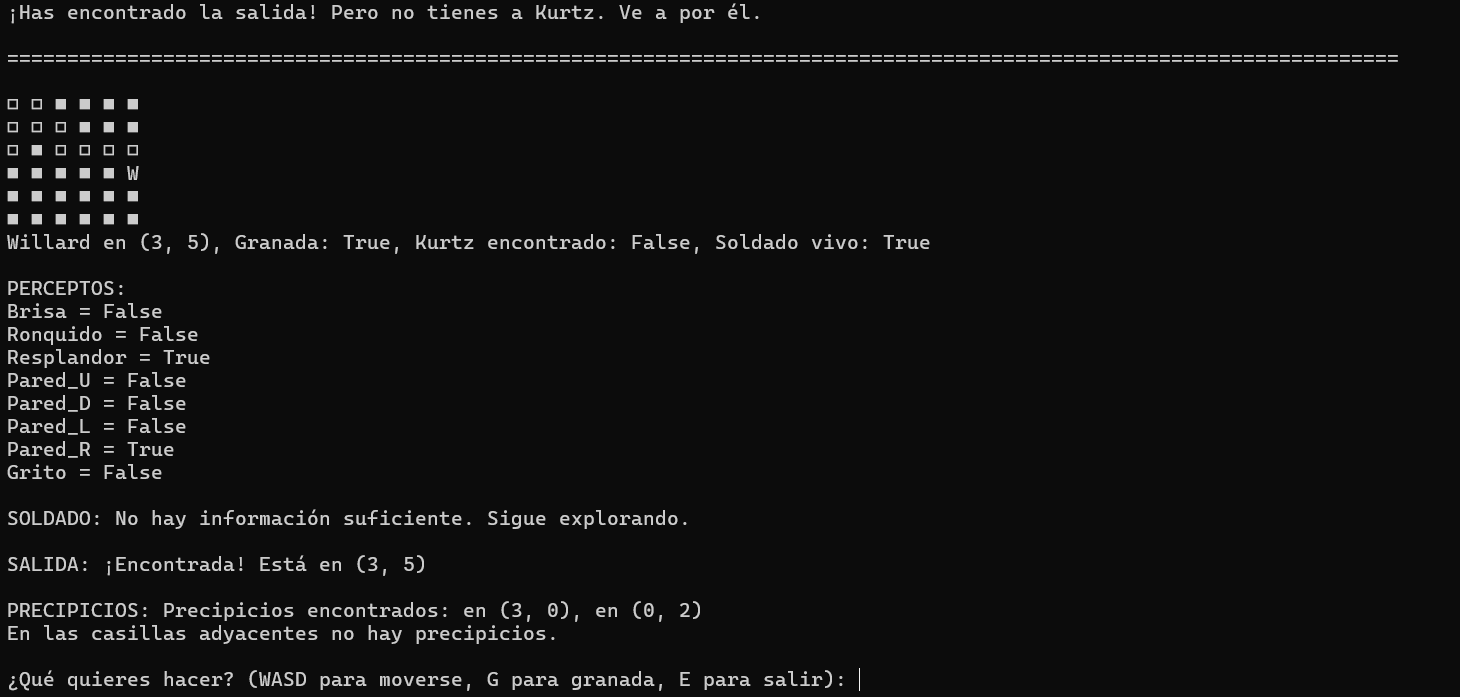
\includegraphics[width=0.85\linewidth]{figs/p1_turno.png}
\caption{Parte 1: ejemplo de turno completo, con tablero, estado, perceptos, inferencias y petición de acción.}
\end{figure}

En cada turno el jugador ve un mensaje (si ha ocurrido algo, como encontrar a Kurtz o la salida), el tablero (las casillas visitadas aparecen vacías y las desconocidas, rellenas), su estado y la información inferida sobre el soldado, la salida y los precipicios. Para el soldado y la salida, mientras no se haya recibido ningún ronquido o resplandor se indica que no hay información suficiente, ya que pueden estar en cualquier casilla no explorada. A partir de la primera señal, el jugador sabe en todo momento dónde pueden estar, con la dirección si son adyacentes. Para los precipicios se indican los confirmados y las casillas adyacentes que podrían serlo.

\begin{figure}[H]
\centering
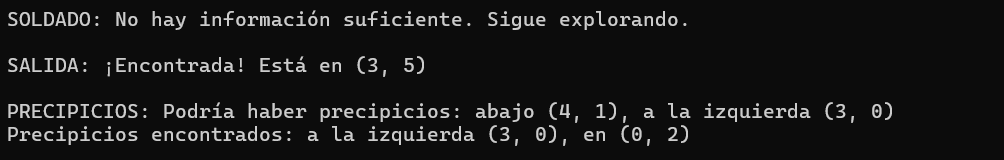
\includegraphics[width=0.8\linewidth]{figs/p1_indicadores.png}
\caption{Parte 1: indicadores de dirección para el soldado, la salida y los precipicios.}
\end{figure}

\subsection{Resultados}
El agente guía al jugador usando solo casillas completamente seguras. En pocos turnos se acota dónde pueden estar el soldado y la salida, y con suficiente exploración se puede llegar a conocer la ubicación de los tres precipicios.

Resulta especialmente interesante el contraste entre un peligro único y tres peligros que emiten la misma señal. Con el soldado y la salida, una señal positiva permite descartar todas las casillas no adyacentes; con los precipicios no, porque la brisa puede deberse a cualquiera de ellos, o incluso a dos a la vez. Por eso, para localizar los tres precipicios hay que explorar prácticamente todo el mapa.

% ================= 4 =================
\section{Parte 2: agente bayesiano}

\subsection{Creencias iniciales}
El agente bayesiano trabaja sobre el palacio de la parte 2 (Tabla~\ref{tab:elementos}). Para cada elemento $X\in\{F, P, D, M, S\}$ mantiene una matriz de creencias de $6\times6$ con la probabilidad $P(X \text{ en } (i,j))$. La distribución inicial es uniforme sobre todas las casillas salvo la de partida: $\pi_{00}=0$ y $\pi_{ij}=1/35$ en las demás.

\begin{figure}[H]
\centering
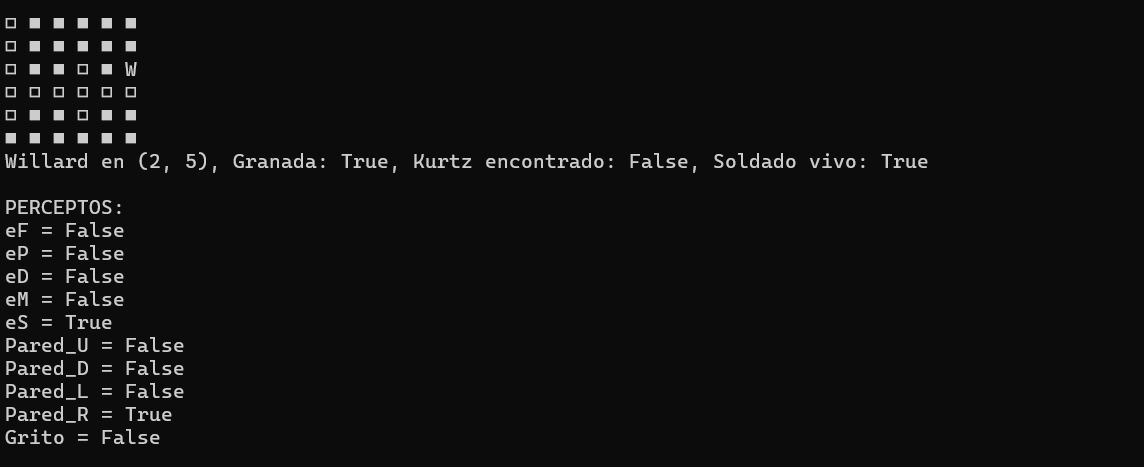
\includegraphics[width=0.7\linewidth]{figs/p2_cuadricula_perceptos.png}
\caption{Parte 2: cuadrícula y perceptos de un turno.}
\end{figure}

\subsection{Actualización con la regla de Bayes}
En cada turno, para cada elemento $X$ y su percepto $e$, se aplica la regla de Bayes en todas las casillas:
\begin{equation}
P(X_{ij}\mid e) \;\propto\; P(e\mid X_{ij})\,P(X_{ij}).
\end{equation}
La verosimilitud es determinista, de acuerdo con el modelo del enunciado. Si el percepto es positivo, vale 1 en las casillas adyacentes a Willard y 0 en el resto; si es negativo, vale 0 en las adyacentes y 1 en el resto. Tras multiplicar por la creencia previa, se normaliza la matriz para que sume 1.

Además, se fuerzan a 0 las probabilidades de todas las casillas visitadas, ya que Willard ha sobrevivido en ellas. Cuando se encuentra la salida, su distribución se concentra en su casilla real. La granada también actualiza las creencias sobre el soldado: si lo mata, su matriz pasa a ser nula; si falla, se anula la casilla objetivo.

\subsection{Riesgo de cada casilla}
Para decidir qué movimientos son seguros, el agente combina las creencias de las tres trampas y del soldado.

\textbf{Probabilidad de trampa.} Las tres trampas se colocan de forma independiente (pueden coincidir en una casilla) y cada percepto depende solo de su propia trampa. Por tanto, las creencias sobre las tres trampas siguen siendo independientes, y la probabilidad de que una casilla contenga al menos una trampa es
\begin{equation}
P(\text{trampa}_{ij}) \;=\; 1-\bigl(1-P(F_{ij})\bigr)\bigl(1-P(P_{ij})\bigr)\bigl(1-P(D_{ij})\bigr).
\end{equation}
Por ejemplo, si un olor a queroseno indica que el fuego está en una de cuatro casillas, cada una tiene una probabilidad de trampa de 0,25.

\textbf{Probabilidad de peligro.} El soldado nunca se coloca en una casilla con trampa, así que los sucesos «hay una trampa» y «está el soldado» son incompatibles, y la probabilidad de peligro es su suma:
\begin{equation}
P(\text{peligro}_{ij}) \;=\; P(\text{trampa}_{ij}) + P(M_{ij}).
\end{equation}
Un movimiento se considera seguro si la casilla de destino tiene $P(\text{peligro}) < 0{,}1$. Si ningún movimiento cumple esta condición, el agente indica cuál es el menos arriesgado y su probabilidad de peligro.

\subsection{Mapas de calor}
A partir de las creencias actualizadas se dibujan tres mapas de calor con \code{seaborn}: la probabilidad de que haya alguna trampa en cada casilla, la probabilidad del soldado y la probabilidad de la salida. Cada casilla muestra su valor numérico, y la posición de Willard se marca con un círculo azul.

\begin{figure}[H]
\centering
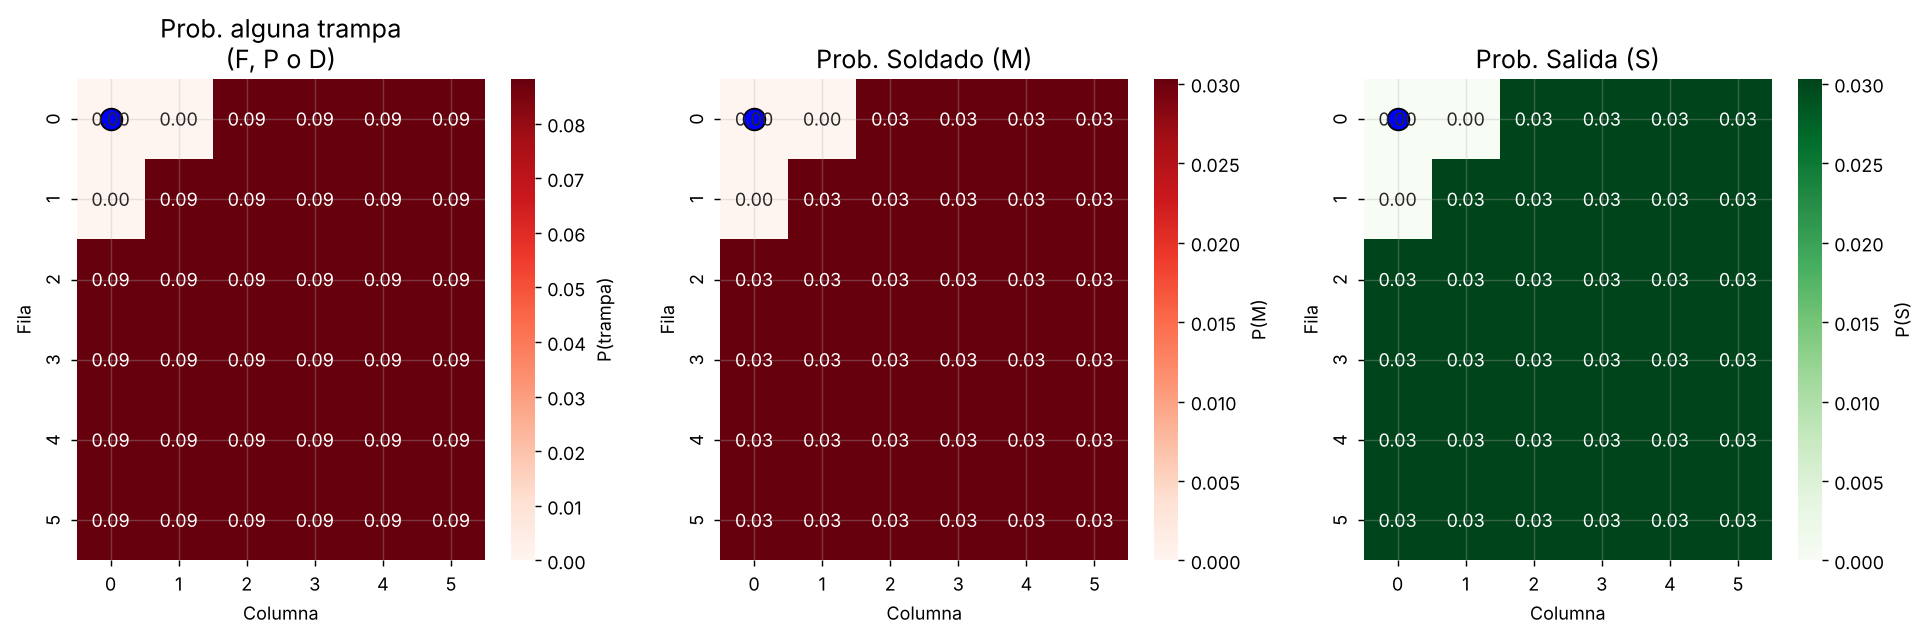
\includegraphics[width=\linewidth]{figs/heatmaps_turno1.png}
\caption{Mapas de calor en el primer turno de una partida. Los perceptos negativos anulan el peligro en las casillas adyacentes.}
\end{figure}

\begin{figure}[H]
\centering
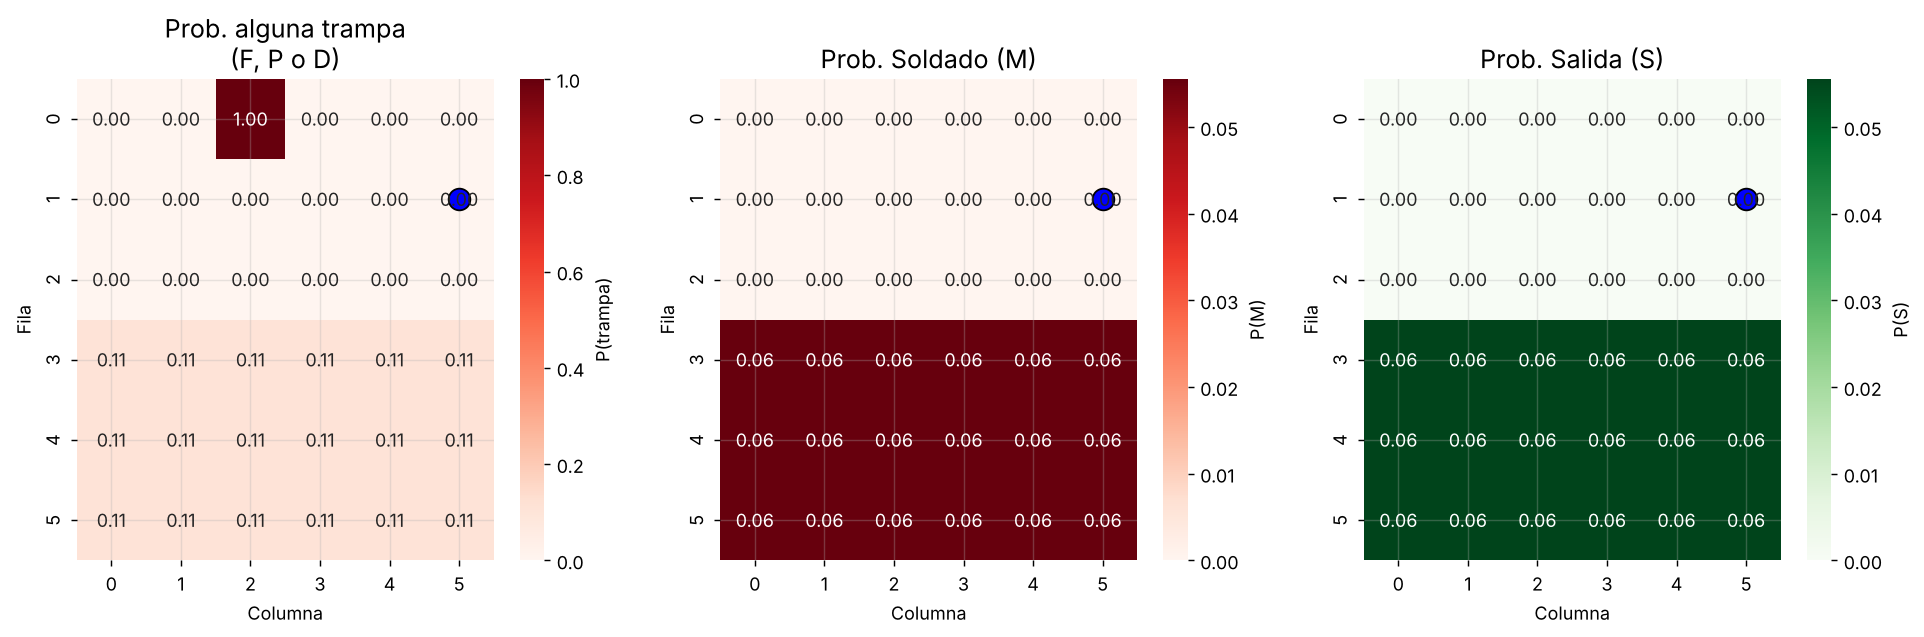
\includegraphics[width=\linewidth]{figs/heatmaps_turno9.png}
\caption{Mapas de calor en el turno 9 de la misma partida. El agente ha localizado con certeza la trampa de pinchos en $(0,2)$, y las casillas que siguen sin explorar tienen una probabilidad de trampa de 0,11.}
\end{figure}

\subsection{Flujo de ejecución}
Cada turno sigue los siguientes pasos:
\begin{enumerate}
\item Se imprime la cuadrícula: solo se ven las casillas visitadas y la posición de Willard.
\item Se calculan y muestran los perceptos de la casilla actual.
\item Se actualizan las creencias con \code{update\_beliefs()}.
\item Se dibujan los tres mapas de calor.
\item Se calculan y muestran los movimientos seguros.
\item El jugador elige su acción: moverse, lanzar la granada o intentar salir.
\end{enumerate}

\begin{figure}[H]
\centering
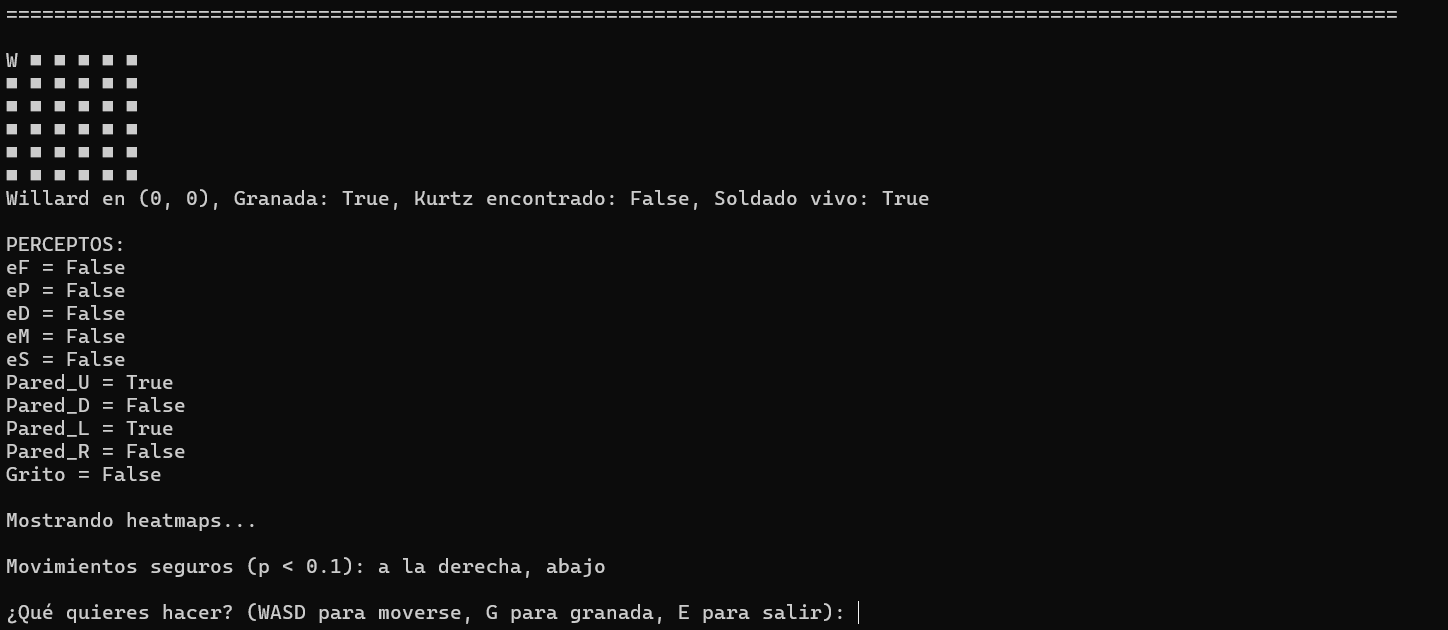
\includegraphics[width=0.85\linewidth]{figs/p2_turno.png}
\caption{Parte 2: salida completa de un turno.}
\end{figure}

\subsection{Resultados}
La inferencia bayesiana refina las creencias de forma intuitiva. Un percepto positivo como \code{eM} anula la probabilidad del soldado en todo el tablero salvo en las casillas adyacentes, que pasan a repartirse la probabilidad (entre 0,25 y 0,5 cada una, según cuántas casillas adyacentes haya). Un percepto negativo anula el elemento en las casillas adyacentes y eleva ligeramente la probabilidad del resto; por ejemplo, en el primer turno pasa de $1/35\approx0{,}029$ a $1/33\approx0{,}030$.

Con un umbral de 0,1 el agente es conservador: solo recomienda casillas en las que los perceptos han descartado prácticamente todo peligro. Una casilla sin ninguna información tiene una probabilidad de peligro de entre 0,11 y 0,12 al principio de la partida (tres trampas y un soldado repartidos entre las casillas restantes), por lo que nunca se considera segura sin evidencia.

% ================= 5 =================
\section{Parte 3: proceso de decisión de Markov}

\subsection{El río}
El capitán y Kurtz deben cruzar un río representado por una cuadrícula de 7 filas y 6 columnas. Las columnas de los extremos son orillas sin corriente; en cada columna interior la corriente tiene una intensidad aleatoria $rs_j\in[0{,}06;\ 0{,}94]$ que empuja hacia abajo. En el río hay dos islas en posiciones aleatorias, y la salida se sitúa en una fila aleatoria de la orilla derecha. El capitán empieza en $(0,0)$.

\subsection{Componentes del MDP}
\begin{itemize}
\item \textbf{Estados:} las casillas de la cuadrícula que no son islas.
\item \textbf{Acciones:} $\mathcal{A}=\{\text{up}, \text{down}, \text{left}, \text{right}\}$. La acción «quedarse» no se elige: aparece cuando un movimiento choca con un borde o con una isla.
\item \textbf{Transiciones:} con una acción distinta de \emph{down}, el capitán se mueve en la dirección elegida con probabilidad $1-rs_j$ y la corriente lo arrastra hacia abajo con probabilidad $rs_j$. La acción \emph{down} es determinista. Si un movimiento choca con un borde o con una isla, el capitán se queda en su casilla, y esa probabilidad se acumula en «quedarse».
\item \textbf{Recompensas:} $R(s')=+100$ al llegar a la salida y $-1$ por cada paso, para minimizar su número. El código define también $-100$ para las islas, pero no llega a aplicarse: como un movimiento hacia una isla deja al capitán en su casilla, las islas actúan como obstáculos, y chocar con ellas solo cuesta un paso.
\item \textbf{Estado terminal:} la salida. La partida acaba al alcanzarla, por lo que su valor es 0 y la recompensa de $+100$ se recibe al entrar en ella.
\item \textbf{Factor de descuento:} $\gamma=0{,}95$.
\end{itemize}

\subsection{Value iteration}
La política óptima se obtiene iterando la ecuación de Bellman desde $V_0(s)=0$:
\begin{equation}
V_{k+1}(s) \;=\; \max_{a\in\mathcal{A}} \sum_{s'} P(s'\mid s,a)\,\bigl[R(s')+\gamma\,V_k(s')\bigr].
\end{equation}
Para cada estado se calcula $Q(s,a)$ para las cuatro acciones, se toma $V(s)=\max_a Q(s,a)$ y se guarda la acción que alcanza el máximo como $\pi(s)$. Los valores se actualizan sobre la misma matriz a medida que se recorren los estados, una variante que converge al mismo punto fijo. El algoritmo se detiene cuando ningún valor cambia más de $\theta=10^{-6}$ entre dos iteraciones.

\begin{figure}[H]
\centering
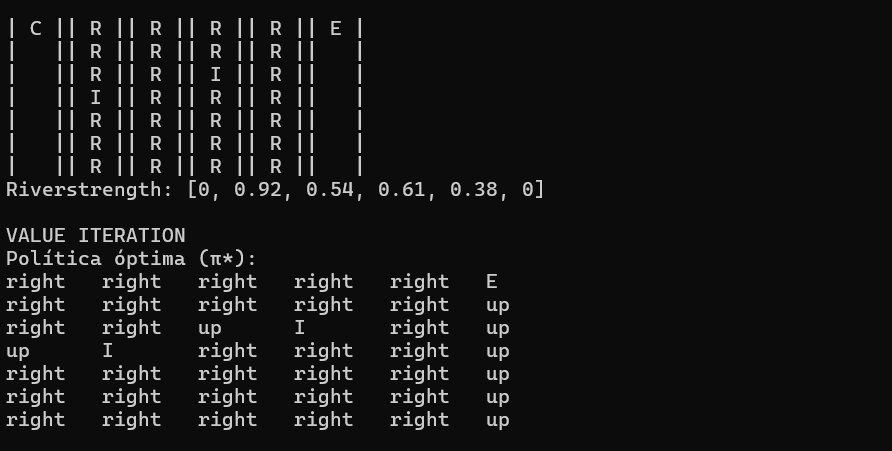
\includegraphics[width=0.62\linewidth]{figs/p3_rio_politica.png}
\caption{Ejemplo de río (C: capitán, R: río, I: isla, E: salida), intensidad de la corriente por columna y política óptima $\pi^*$.}
\end{figure}

\subsection{Simulación}
Con la política óptima se simulan diez partidas desde $(0,0)$. En cada paso se aplica la acción $\pi^*(s)$ y se sortea el estado siguiente según $P(s'\mid s,a)$. Se muestra si el movimiento se debe a la corriente y la recompensa acumulada. Como cada paso cuesta 1 y la salida da 100, la recompensa de una partida de $k$ pasos es $100-(k-1)$.

\begin{figure}[H]
\centering
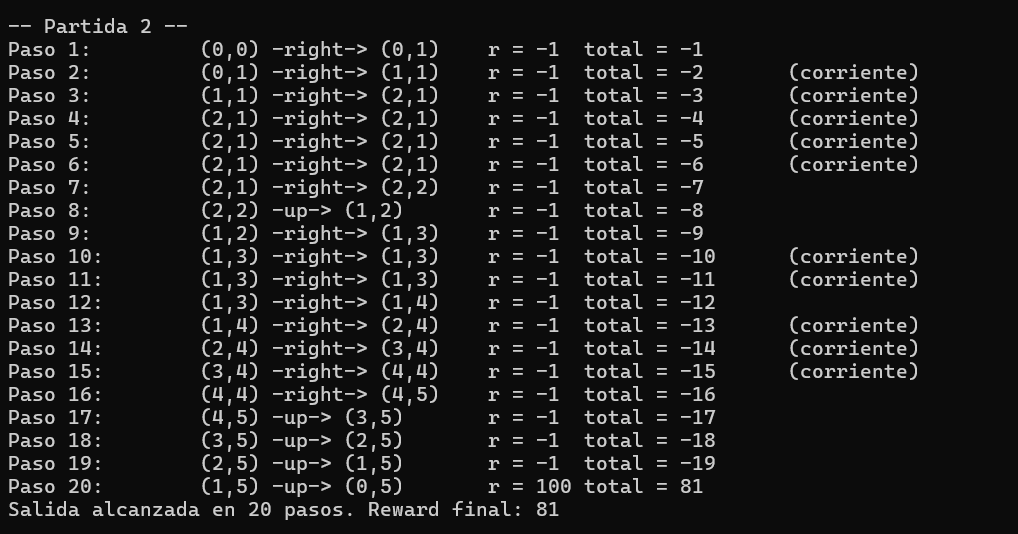
\includegraphics[width=0.68\linewidth]{figs/p3_simulacion.png}
\caption{Simulación de una partida con la política óptima.}
\end{figure}

\subsection{Resultados}
Para caracterizar el comportamiento del programa se ha ejecutado sobre 200 ríos generados aleatoriamente (Tabla~\ref{tab:mdp}).

\begin{table}[H]
\centering\small
\caption{Resultados del MDP sobre 200 ríos aleatorios.}\label{tab:mdp}
\begin{tabular}{@{}lc@{}}
\toprule
\textbf{Magnitud} & \textbf{Valor}\\
\midrule
Iteraciones hasta la convergencia & mediana 73 (entre 19 y 172)\\
Valor óptimo del estado inicial, $V^*(0,0)$ & mediana 40,5 (entre 4,6 y 64,1)\\
Recompensa media de 10 partidas & mediana 86,9 (el 80 \% de los ríos, entre 73,5 y 91,1)\\
Pasos por partida & media 16,9; mediana 13\\
\bottomrule
\end{tabular}
\end{table}

La política óptima hace lo que cabe esperar de ella: evita chocar con las islas, que solo harían perder pasos, tiende a ir hacia la derecha cuando puede y, para rodear una isla, sube por las columnas con poca corriente y baja por las de corriente fuerte. Aprovecha las columnas en las que es menos probable que la corriente lo arrastre para ganar altura, y deja que la corriente actúe donde la caída es menos perjudicial.

% ================= 6 =================
\section{Conclusiones}

Los tres programas muestran tres formas de razonar en un mismo escenario. El agente lógico trabaja con certezas: solo afirma lo que se deduce de los perceptos, lo que lo hace fiable pero limitado cuando varios peligros producen la misma señal. El agente bayesiano cuantifica la incertidumbre y permite decidir con un nivel de riesgo controlado; para ello es esencial combinar correctamente las creencias, teniendo en cuenta qué elementos son independientes y cuáles incompatibles. Finalmente, el MDP del río introduce la toma de decisiones secuencial con transiciones estocásticas: \emph{value iteration} encuentra una política que aprovecha o evita la corriente según la columna, y en la mitad de las partidas simuladas llega a la salida en 13 pasos o menos.

\end{document}
